
O setor de jogos digitais está em constante expansão, projetando ultrapassar os US\$ 200 bilhões em 2023, conforme previsto por \citeonline{quanto_games_vao_movimentar}. A plataforma Steam, em 2022, testemunhou o lançamento de 10.644 novos títulos, e até 6 de outubro de 2023, esse número alcançou 9.103, indicando uma notável tendência crescente, conforme revelado pela \cref{fig:steam_publishes}.

\begin{figure}[!ht]
\centering
\caption{Número de jogos publicados na Steam.}
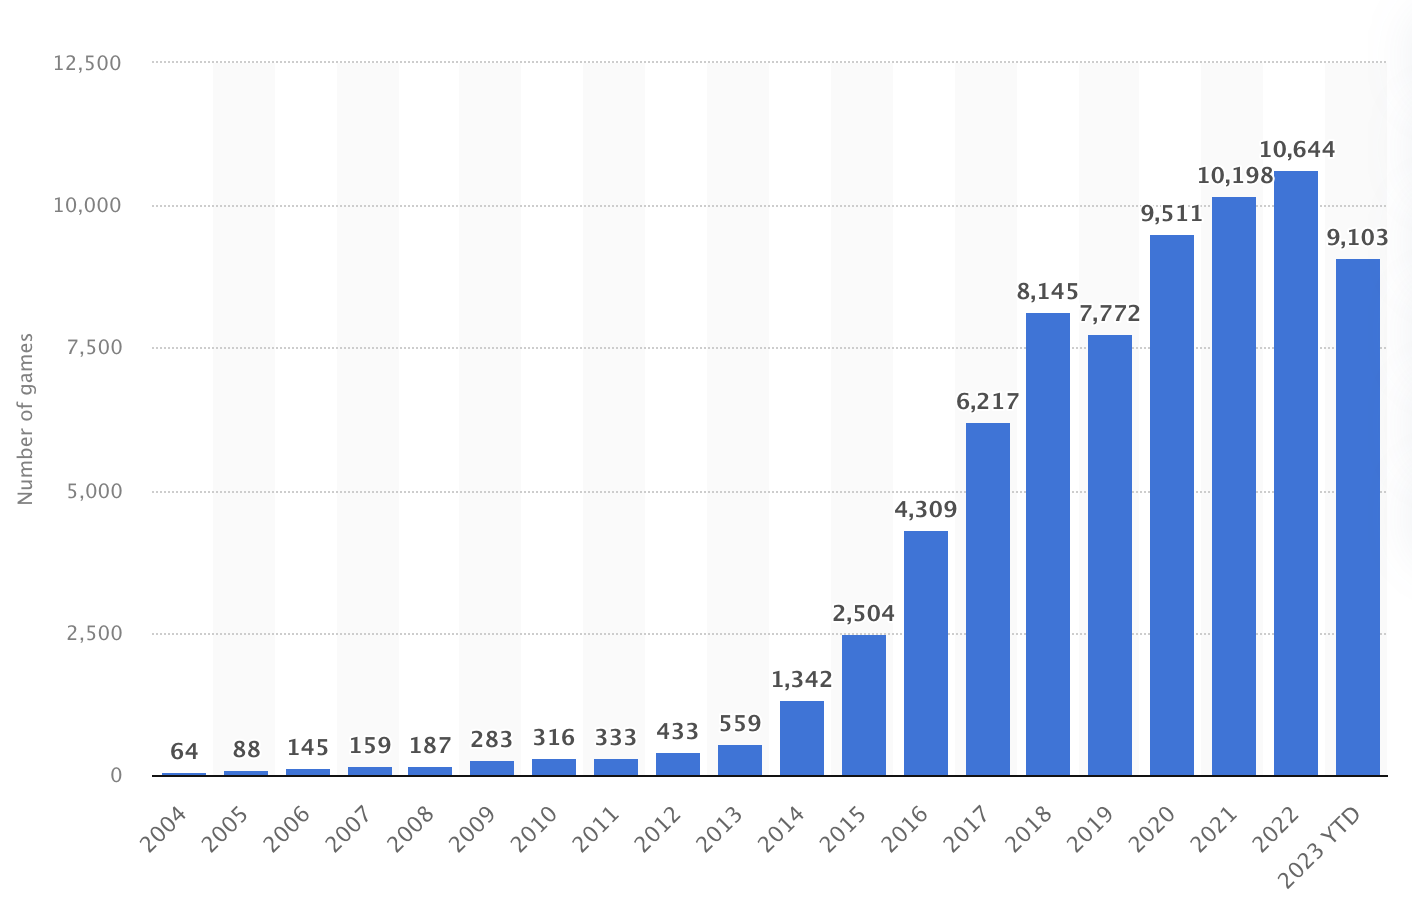
\includegraphics[width=0.6\textwidth]{figures/steam_sales.png}
\legend{Fonte: \citeonline{numero_de_jogos_publicados_na_steam}}
\label{fig:steam_publishes}
\end{figure}

No contexto dos jogos, os mapas desempenham um papel crucial, guiando os jogadores e enriquecendo suas experiências ao proporcionar uma sensação de escala e fomentar uma exploração mais rica \cite{video_game_maps, minimap}.

A elaboração de mapas no universo dos jogos utiliza a técnica de geração procedural, fundamentada na criação dinâmica de conteúdo por meio de algoritmos. Inicialmente concebida para superar desafios de armazenamento, a geração procedural persiste como uma estratégia para criar conteúdos exclusivos a cada execução do programa \cite{kenny2021procedural, lambda3}.

Dentro dessa abordagem, diversas técnicas são exploradas, desde o \textit{Perlin Noise} para criar contornos e texturas naturais, os \textit{L-systems} para gerar vegetação, até o \textit{Voronoi} para criar texturas e particionar espaços 2D, e os autômatos celulares para criar cavernas em 2D, entre outras abordagens \cite{kvrivzmulti}.

Nesse contexto de geração procedural de mapas, surgem desafios consideráveis, conforme discutido por \citeonline{geracao_procedural_jogos_2d}: "Um dos maiores desafios no desenvolvimento de algoritmos para geração de mapas é a dificuldade de criar cenários que sejam, ao mesmo tempo, atraentes e diversificados, permitindo que o jogador possa explorar um novo ambiente a cada sessão de jogo" \cite{geracao_procedural_jogos_2d}.

Para criar mapas diversificados, propomos estabelecer um escopo inspirado no jogo \textit{Minecraft}, conhecido por gerar mapas proceduralmente com biomas que incluem diferentes características, como flora, fauna, relevo, temperaturas e umidade \cite{mojang}. Nesse escopo, pretendemos gerar mapas com biomas utilizando a abordagem proposta por \citeonline{amitp2010}, que utiliza o diagrama de Voronoi para particionar em regiões atribuíveis a diferentes biomas.

Adicionalmente, visando adicionar personalização e enriquecer a diversidade, planejamos implementar uma funcionalidade que permita a definição do contorno do mapa por meio da segmentação de uma imagem, originada de desenhos ou de contextos cotidianos. Para isso, empregaremos técnicas de segmentação, as quais, conforme afirmado por \citeonline{saiwa}, simplificam a representação ao dividir a imagem em regiões com base em características como cor, textura ou forma. Essas técnicas, úteis para rastreamento e reconhecimento de objetos, possibilitarão a segmentação de desenhos, utilizando, por exemplo, o preenchimento por inundação. Além disso, incorporaremos modelos de inteligência artificial (IA) para a segmentação de cenários mais complexos, abrangendo elementos como pessoas e veículos \cite{saiwa, OpenCVFloodFill, dp_semantic_segmantation}.

Portanto, o escopo de nossa pesquisa abrange a geração procedural de mapas com biomas, permitindo a escolha do contorno a partir de um desenho com técnicas de segmentação ou da segmentação de uma imagem mais complexa com modelos de IA. Esta aplicação viabilizará aos desenvolvedores a incorporação dessa nova funcionalidade em um jogo em fase de desenvolvimento, proporcionando ao usuário final a opção de selecionar ou capturar uma foto e escolher um contorno específico para gerar um mapa contendo os biomas.

Com o intuito de contribuir cientificamente, formulamos a hipótese de que quanto mais pontos o diagrama de Voronoi tiver, maior será a precisão na compatibilidade entre o mapa gerado e o contorno escolhido. Para testar essa hipótese, serão realizados testes com métricas para avaliar a qualidade da geração procedural com o contorno selecionado. Além disso, será realizado um conjunto de testes com métricas específicas para verificar a hipótese formulada: a relação direta entre a precisão na compatibilidade entre o mapa gerado e o contorno escolhido e o número de pontos no diagrama de Voronoi.

\section{Objetivos}

O objetivo principal deste trabalho é abordar um desafio inerente ao desenvolvimento de jogos digitais, mais especificamente na geração procedural de mapas. A complexidade está relacionada à criação de cenários que sejam simultaneamente atrativos e heterogêneos, buscando proporcionar aos jogadores experiências distintas a cada sessão de jogo. A solução proposta visa aprimorar essa capacidade, concentrando-se na habilidade de identificar contornos em imagens derivadas de desenhos ou cenas cotidianas. Essa abordagem pretende possibilitar a criação de mapas contendo biomas com base nos limites predefinidos pelo usuário, visando, assim, a ampliação da diversidade e personalização dos ambientes virtuais, com potencial impacto positivo na experiência do jogador.

Adicionalmente, os seguintes objetivos específicos serão abordados:

\begin{itemize}
	\item Selecionar conjuntos de dados contendo classes relevantes, como pessoas, carros, entre outros, para treinar um modelo IA específico para a segmentação de imagens.
	\item Utilizar algoritmos para criar diagrama de Voronoi.
	\item Aplicar um algoritmo para reconhecer a imagem com o contorno selecionado e gerar, como resultado, a imagem do mapa gerado.
	\item Utilizar o resultado da segmentação para indicar o que é terreno sobre o diagrama de Voronoi.
	\item Gerar os biomas no diagrama de Voronoi.
	\item Criar testes com o intuito de mensurar a semelhança entre o contorno do mapa gerado e o contorno escolhido.
\end{itemize}